

\chapter{Sperimentazione di attacco di linking}

La dimostrazione in questione simula un \textbf{attacco di linking} tra un \textbf{dataset pseudonimizzato} e un dataset contenente dati non anonimizzati. L'attacco riesce perché nei due dataset sono presenti \textbf{corrispondenze tra soggetti} riguardo attributi come:

\begin{itemize}
  \item Età
  \item Genere
  \item Gruppo sanguigno
\end{itemize}

Tramite l'utilizzo di \textbf{Python} e \textbf{Jupyter Notebook} ho creato il seguente esempio di attacco.

\newpage

\section{Dataset di Informazioni Mediche sui Cittadini Americani}

In questa fase iniziale, procediamo alla visualizzazione di un dataset contenente informazioni mediche di cittadini americani. Il dataset è gratuito ed è stato scaricato dalla piattaforma Kaggle. Può essere trovato al seguente link: \href{https://www.kaggle.com/datasets/prasad22/healthcare-dataset?resource=download}{https://www.kaggle.com/datasets/prasad22/healthcare-dataset?resource=download} e include le seguenti informazioni sui pazienti:

\begin{itemize}
  \item \textbf{Name}: Nome del paziente associato al record sanitario.
  \item \textbf{Age}: Età del paziente al momento dell'ammissione, espressa in anni.
  \item \textbf{Gender}: Genere del paziente, può essere "Maschio" o "Femmina".
  \item \textbf{Blood Type}: Gruppo sanguigno del paziente, come "A+", "O-", eccetera.
  \item \textbf{Medical Condition}: Condizione medica primaria o diagnosi associata al paziente, come "Diabete", "Ipertensione", "Asma", e altre.
  \item \textbf{Date of Admission}: Data di ammissione del paziente presso la struttura sanitaria.
  \item \textbf{Doctor}: Nome del medico responsabile delle cure durante l'ammissione del paziente.
  \item \textbf{Hospital}: Identifica l'ospedale o la struttura sanitaria dove il paziente è stato ammesso.
  \item \textbf{Insurance Provider}: Fornitore dell'assicurazione del paziente, che può essere tra diversi opzioni come "Aetna", "Blue Cross", "Cigna", "UnitedHealthcare" e "Medicare".
  \item \textbf{Billing Amount}: Importo fatturato per i servizi sanitari forniti al paziente durante l'ammissione, espressa come numero decimale.
  \item \textbf{Room Number}: Numero della stanza dove il paziente è stato alloggiato durante l'ammissione.
  \item \textbf{Admission Type}: Specifica il tipo di ammissione, come "Emergenza", "Elettiva" o "Urgente", riflettendo le circostanze dell'ammissione.
  \item \textbf{Discharge Date}: Data di dimissione del paziente dalla struttura sanitaria, basata sulla data di ammissione e un numero casuale di giorni entro un intervallo realistico.
  \item \textbf{Medication}: Identifica una medicazione prescritta o somministrata al paziente durante l'ammissione, come "Aspirina", "Ibuprofene", "Penicillina", "Paracetamolo" e "Lipitor".
  \item \textbf{Test Results}: Descrive i risultati di un test medico eseguito durante l'ammissione del paziente. Possibili valori includono "Normale", "Anormale" o "Inconcludente".
\end{itemize}

Il dataset contiene un totale di 55,500 record.

\section{Visualizzazione del Dataset}

Il seguente codice Python mostra come leggere e visualizzare i primi cinque record del dataset utilizzando la libreria \texttt{pandas}:\\

\begin{lstlisting}[caption={Visualizzazione dataset}]
import pandas as pd

pd.set_option("display.max_columns", None)  
file_path = "Allegati/healthcare_dataset.csv"
df = pd.read_csv(file_path)

display(df.head())  # Stampa solo i primi 5 record
\end{lstlisting}

\begin{figure}[H]
    \centering
    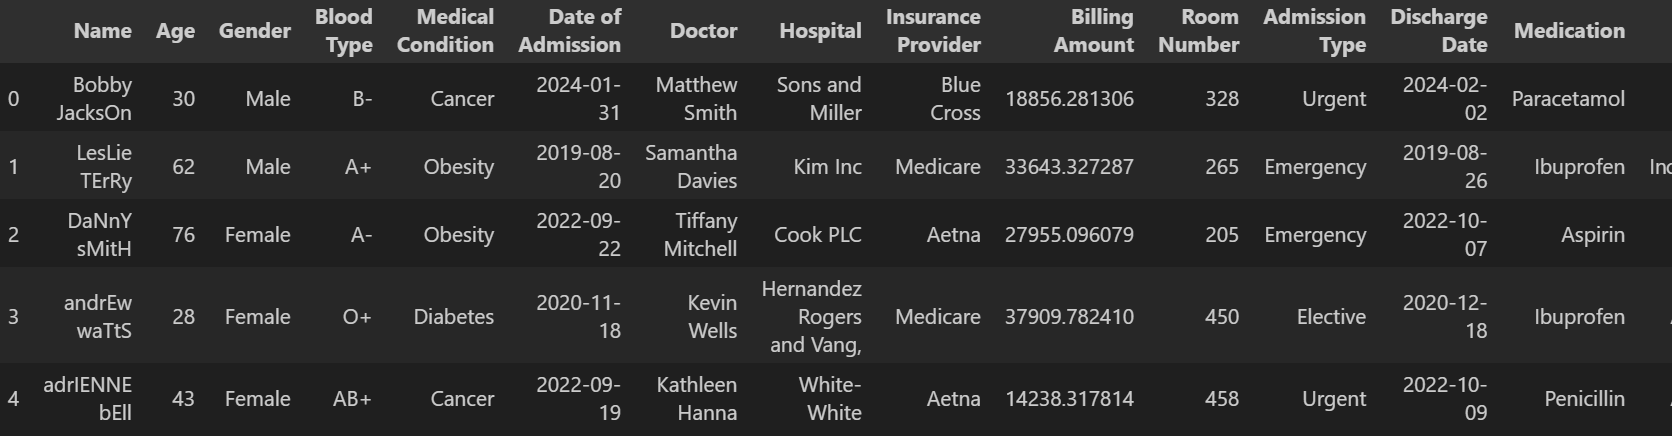
\includegraphics[width=1.0\linewidth]{Images/Img1.png}
    \caption{Dataset originale}
\end{figure}

\section{Pseudonimizzazione del Dataset}

In questa fase, si vogliono proteggere le informazioni sensibili del dataset come il nominativo del paziente per rendere il dataset pseudo-anonimizzato. Utilizziamo la tecnica di sostituire il nominativo della persona creando una funzione che sostituisce il nome tramite la seguente operazione matematica:

\[
\text{newName} = \sum_{i=1}^{n} \text{ASCII}(c_i) + \text{Room Number}
\]

dove:

\begin{itemize}
    \item \(c_i\) sono i caratteri di \textit{oldName}
    \item \(\text{ASCII}(c_i)\) rappresenta il valore ASCII del carattere \(c_i\)
\end{itemize}

Tronchiamo inoltre il dataset a soli 1000 valori per velocizzare le operazioni successive. \\


\begin{lstlisting}[caption={Visualizzazione dataset}]
output_file = "Allegati/truncated_dataset.csv"
df.head(1000).to_csv(output_file, index=False) 

new_dataframe = pd.read_csv(output_file)

# Somma dei valori ASCII dei caratteri in 'name'
def pseudonimize(name, room):
    name_ascii_sum = sum(ord(char) for char in name) 
    return name_ascii_sum + room
    
for index, row in new_dataframe.iterrows():
    new_name = pseudonimize(row["Name"], row["Room Number"])
    new_dataframe.loc[index, "Name"] = new_name

display(new_dataframe.head())
\end{lstlisting}

\begin{figure}[H]
    \centering
    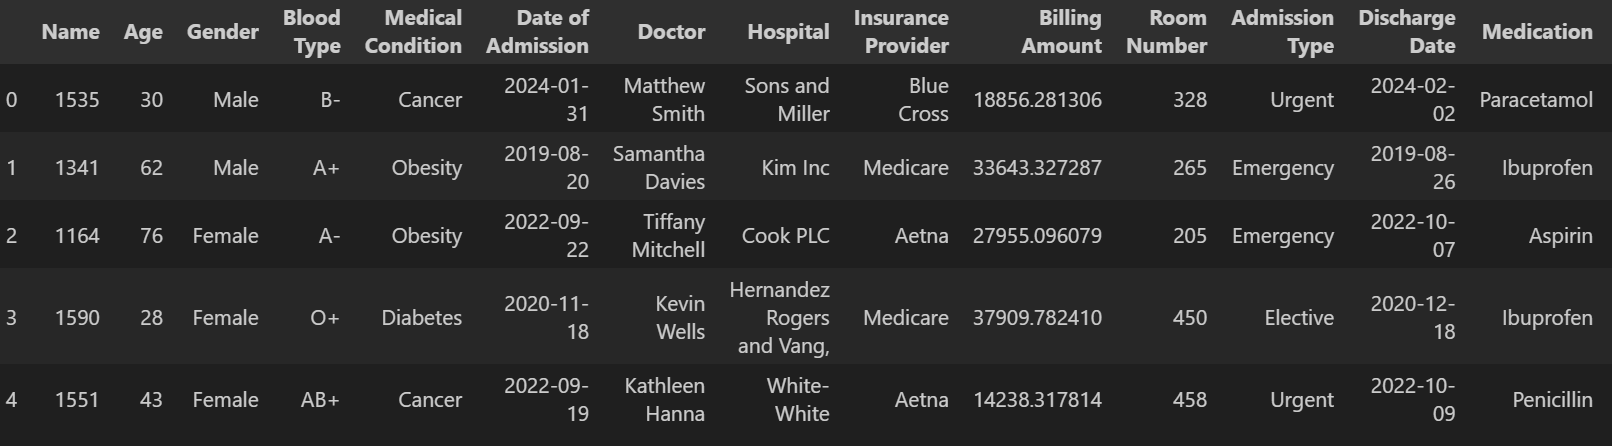
\includegraphics[width=0.95\linewidth]{Images/Img2.png}
    \caption{Dataset pseudonimizzato}
\end{figure}

\section{Creazione di un meccanismo di recupero}

Quando pseudonimizziamo un dataset e abbiamo bisogno successivamente di risalire al nominativo originale del paziente, è necessario creare una \textbf{tabella di mappatura} tra il nominativo del paziente e il suo pseudonimo. Questa tabella deve essere conservata in modo sicuro e protetto poiché contiene tutte le coppie tra nominativo e pseudonimo presenti nel dataset pseudonimizzato.\\

\begin{lstlisting}[caption={Creazione Tabella di Mappatura}]
df_nomi = df['Name'].head(1000)
new_df_nomi = new_dataframe['Name'].head(1000)

# Creiamo un nuovo dataframe con i nomi ottenuti
nomi_dataframe = pd.DataFrame({
    'Nome': df_nomi,
    'Nome Pseudonimizzato': new_df_nomi
})

# Scriviamo il dataframe in un file CSV
nomi_dataframe.to_csv('Allegati/tabellaMappatura.csv', index=False)

display(nomi_dataframe.head())
\end{lstlisting}

\begin{figure}[H]
    \centering
    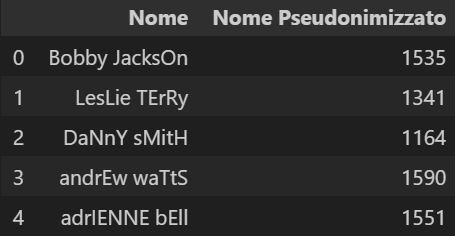
\includegraphics[width=0.95\linewidth]{Images/Img3.png}
    \caption{Dataset pseudonimizzato}
\end{figure}

\section{Inizio dell'attacco di linking}

Durante questa fase, l'attaccante dispone di due dataset cruciali:

\begin{itemize}
    \item Il file \texttt{pseudonymized.csv} che contiene informazioni sanitarie di vari pazienti, con i loro nominativi pseudonimizzati.
    \item Il file \texttt{blood\_donation\_dataset.csv} che include dettagli su donatori di sangue, specificamente:
    
    \begin{itemize}
        \item \textbf{Nome}: Il nome completo del donatore di sangue.
        \item \textbf{Età}: L'età del donatore al momento della donazione.
        \item \textbf{Genere}: Il genere del donatore, indicato come "Maschio" o "Femmina".
        \item \textbf{Gruppo Sanguigno}: Il tipo di sangue del donatore.
        \item \textbf{Data della Donazione}: La data in cui è stata effettuata la donazione.
    \end{itemize}
\end{itemize}

L'obiettivo dell'attacco è ricondurre all'identificazione dei pazienti all'interno del dataset pseudonimizzato, sfruttando le informazioni disponibili nel dataset delle donazioni di sangue che contiene i nomi completi in chiaro. \\

\begin{lstlisting}[caption={Dataset Donatori di sangue}]
file_path = "Allegati/blood_donation_dataset.csv"
blood_donation = pd.read_csv(file_path)

display(blood_donation.head())
\end{lstlisting}

\begin{figure}[H]
    \centering
    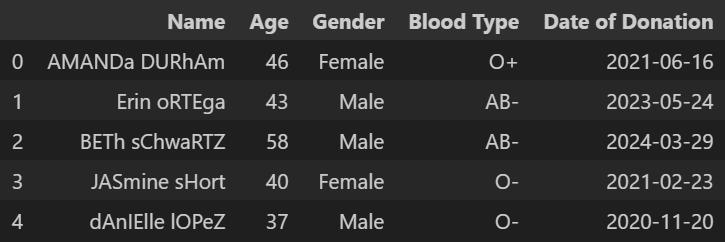
\includegraphics[width=0.95\linewidth]{Images/Img4.png}
    \caption{Dataset donatori di sangue}
\end{figure}

\newpage
Supponiamo adesso di voler trovare il nominativo associato alla entry \textbf{n°546} del nostro dataset anonimizzato\\

\begin{lstlisting}[caption={Ricerca pseudonimo}]
file_path = "Allegati/pseudonymized.csv"
pseudonymized = pd.read_csv(file_path)

# Modificare questo valore per cercare un altro utente
indiceDaCercare = 546 

display(pseudonymized.iloc[indiceDaCercare].to_frame().T)
\end{lstlisting}

\begin{figure}[H]
    \centering
    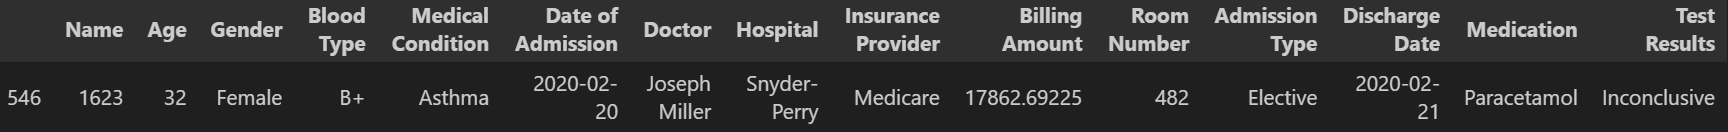
\includegraphics[width=1.0\linewidth]{Images/Img5.png}
    \caption{Dataset donatori di sangue}
\end{figure}

Dalla seguente voce, possiamo estrarre informazioni utili come:

\begin{itemize}
    \item Età: 32 anni
    \item Genere: Femmina
    \item Gruppo Sanguigno: B+
\end{itemize}

Queste informazioni sono fondamentali per condurre un attacco di collegamento tramite il nostro dataset \texttt{blood\_donation\_dataset.csv}. 

Ora cerchiamo un record che soddisfi tutte e tre queste condizioni.\\

\begin{lstlisting}[caption={Attacco di linking}]
def search(age, gender, bloodType):
    for index, row in blood_donation.iterrows():
        if (
            row["Age"] == age
            and row["Gender"] == gender
            and row["Blood Type"] == bloodType
        ):
            return index
        
age = pseudonymized.iloc[indiceDaCercare]["Age"]
gender = pseudonymized.iloc[indiceDaCercare]["Gender"]
bloodType = pseudonymized.iloc[indiceDaCercare]["Blood Type"]

result = search(age, gender, bloodType)
display(blood_donation.iloc[result].to_frame().T)
\end{lstlisting}

\newpage

\begin{figure}[H]
    \centering
    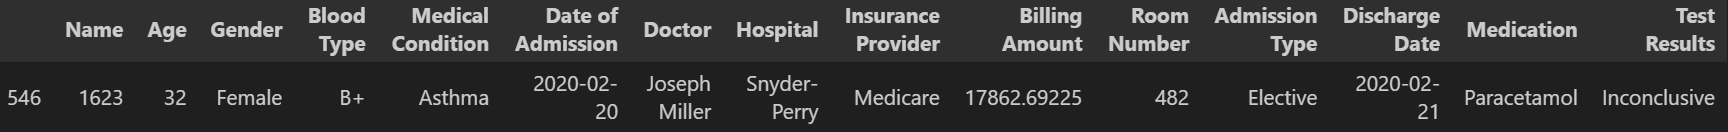
\includegraphics[width=1.0\linewidth]{Images/Img5.png}
    \caption{Output attacco di linking}
\end{figure}

\section{Conclusione dell'attacco di linking}

L'attacco di linking ha identificato un record di una donatrice chiamata "Connor BARTOn" che sembra corrispondere al paziente cercato. Supponiamo che l'attaccante conosca l'algoritmo utilizzato per la pseudonimizzazione.

Per verificare la corrispondenza, sottraiamo il numero della stanza dal nome pseudonimizzato del paziente, ottenendo la somma dei caratteri ASCII del nome. Confrontiamo poi questa somma con quella del nome trovato nel dataset originale.\\

\begin{lstlisting}[caption={Conclusione attacco di linking}]
# Somma dei caratteri ASCII del nome nel database pseudonimizzato
check = pseudonymized.iloc[indiceDaCercare]["Name"] - pseudonymized.iloc[indiceDaCercare]["Room Number"]

# Nome trovato nel DataFrame blood_donation
nomeTrovato = blood_donation.iloc[result]["Name"]

# Calcolo dell'ASCII dei nomi trovati
nomeTrovatoASCII = sum(ord(char) for char in nomeTrovato)

# Confronto degli ASCII
if nomeTrovatoASCII == check:
    print("Corrispondenza trovata")
else:
    print("Corrispondenza non trovata")
\end{lstlisting}